% 2012 年天津卷理科第 13 题：圆的两条弦 AB、AC，B 处切线与 AC 延长线交于 D，
% CE∥BD 交圆于 E、交 AB 于 F。
% 来源 PDF：普通高考/2012/2012天津理.pdf，第 1 页（印面 775）右栏。
% 按 AF=3、FB=1、EF=3/2 的实际比例作图：A(0,0)，C(4,0)，D(16/3,0)，B(3.5,−1.936)，
% 圆心 (2,−0.516)，半径 2.066；E 为直线 FC 与圆的另一交点（F 在 C、E 之间）。
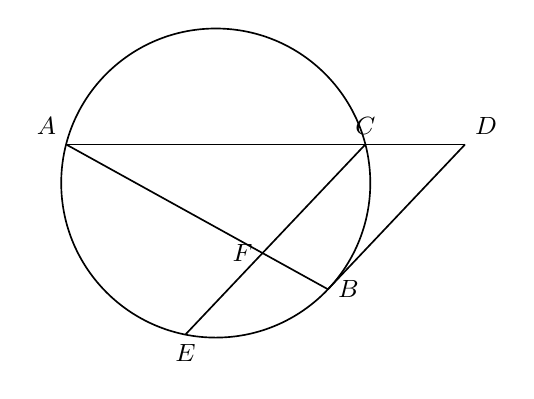
\begin{tikzpicture}[scale=0.95, semithick, font=\small]
  \coordinate (A) at (0,0);
  \coordinate (C) at (4,0);
  \coordinate (D) at (5.333,0);
  \coordinate (B) at (3.5,-1.936);
  \coordinate (F) at (2.625,-1.452);
  \coordinate (E) at (1.594,-2.542);
  \coordinate (O) at (2,-0.516);
  \draw (O) circle (2.066);
  \draw (A) -- (B);
  \draw (A) -- (C);
  \draw (C) -- (D);
  \draw (B) -- (D);
  \draw (E) -- (C);
  \node[above left] at (A) {$A$};
  \node[above] at (C) {$C$};
  \node[above right] at (D) {$D$};
  \node[right] at (B) {$B$};
  \node[left] at (F) {$F$};
  \node[below] at (E) {$E$};
\end{tikzpicture}
